% Chapter 10

\chapter{Results and Discussion} % Chapter title
\label{ch:results}

%----------------------------------------------------------------------------------------

\section{Participant Demographics}

\graffito{Questions are prefixed with a letter indicating which questionnaire they appear in (\textit{I} for initial and \textit{F} for final) followed by the question number. For a detailed look at the questions, please refer to \autoref{an:questionnaires}.}

\noindent A total of 11 participants answered the Call for Participation (see \autoref{sec:online}) and requested a participation link. Of those, one did not attempt to complete the experiment. One further participant completed all experiment parts except filling in the initial questionnaire, so the provided results were not used. Thus, in total 9 participants completed the experiment, which represents 82\,\% of people who requested to participate. Given that one participant mostly completed the experiment and a technical issue may have caused the initial questionnaire not to be saved, that brings the participation rate up to 91\,\%. These figures suggest the approach of asking interested people to request a link and implicitly commit to carrying out the experiment (see \autoref{sec:online}) was effective.

Genderwise, 4 male (44\,\%) and 5 female (56\,\%) participants took part, all in the 20-25 age group. All participants considered themselves native Catalan speakers, while all but one (89\,\%) considered themselves native Spanish speakers (the odd one out did select Spanish as one of the languages he or she speaks). Other languages spoken by the participants include English (100\,\%), French (78\,\%), Spanish (33\,\%), Japanese (22\,\%), German (11\,\%), Italian (11\,\%), Korean (11\,\%), Dutch (11\,\%), Polish (11\,\%) and Catalan (11\,\%). As well as the aforementioned participant, the Spanish and Catalan results are due to a participant selecting them in both the native languages and other languages questions.

All participants have studied translation, during either 4 years (67\,\%) or 5 years (33\,\%) [Question I.9]. Regarding professional experience as translators, 56\,\% reported having worked as translators, while 44\,\% hadn't. Of those that had, 40\,\% had worked for 2 years as a translator, 40\,\% for 1 year and 20\,\% for less than 1 year [Question I.10].

When asked specifically about their professional experience [Question I.11], 56\,\% reported having translated from scratch; 44\,\% reported experience with proof-reading, \ac{PE} and localising; 22\,\% said terminology management, using \ac{CAT} tools and preparing documents for internationalisation; and 11\,\% mentioned transcreation, setting up style guides, \ac{MT} quality evaluation and subtitling. It is interesting to note that the answers to Question 11 and the previous Questions 9 and 10 don't match up as expected, \ie some participants who reported not having worked as translators then went on to say they had professional experience translating from scratch, for example. It is possible that in interpreting the question, participants included internships and odd jobs which they did not fully consider to be ``work''.

Given the previous descriptions, the participants can be classified as semi-professionals: they are no longer students, but still not as experienced as a long-standing professional.


%----------------------------------------------------------------------------------------

\section{Conceptions of Translation}

\noindent This section describes what the participants think about translation [Questions I.1 and I.12--I.23]. The aim of these questions is two-fold. On the one hand, they aim to provide more context for the tool evaluations the participants provide. On the other hand, they aim to verify if translators are a useful source of suggestions of how to improve \ac{CAT} tools.

\subsection{Translation Tasks}

\noindent Participants were asked which tasks they considered boring and which they considered interesting. It is assumed that the boring tasks would be those that a translator would prefer not to do and thus could be considered as a candidate for automation. 

Participants considered that researching and learning about a new topic is one of the most interesting tasks in translation, as well as the process of translation itself [Question I.12]. The problem solving aspect was also frequently mentioned, such as solving cultural clashes and difficulties present in the text. Creativity also came up, a topic which can surprise those who consider translation to be an essentially mechanical task but which is frequently discussed in translation theory. As for what participants found boring when translating [Question I.13], 33\,\% also mentioned topic research. Other aspects considered boring were revising and proofreading, page layout management, terminology research and database management (I interpret this as glossary and translation memory management). One participant even explicitly mentioned \ac{PE} as a boring task.

The questionnaire asked participants that if they could have a tool to automate any task in translation, which task would it be [Question I.14]. A few mentioned the same tasks they considered boring, such as topic research and proofreading. Interestingly, many of the tools they wished for were those that provide suggestions of various kinds: collocations and expressions, synonyms, translation options in context and problematic structures in the text. This suggests participants wished to remain in control of their translations and have the power to pick an option, rather than being forced an option in the case of \ac{TM} and \ac{PE} which they then have to change only if necessary (as most \ac{PE} guidelines state, see for example \textcite{carl2015post}). 

Thus, it appears that simple questionnaires asking translators what tasks they would like to be automated is a useful way to come up with \ac{CAT} tool improvements. It also shows that not all improvements can please everyone: one participant stated they had all the tools they needed to translate while another explicitely mentioned \ac{PE} as an activity they dislike.


\subsection{What Makes a Good Translation}

\noindent The question of translation evaluation ---what a good and a bad translation is, if they can even be classified as such--- is inextricably linked to how translation is conceptualised. Participants were asked what translation meant to them [Question I.1]. To analyse the responses, the translation theory paradigms discussed in \autoref{sec:paradigms} provide a good starting point. Given the freeform answers and open-ended question, it is difficult to classify a participant's views in one paradigm or the other. However, a large number of responses describe translation in a similar fashion to the equivalence paradigm, some nuancing this description with tints of functional priorities and the need to adapt the text to the target culture and function. 

To garner a more detailed and nuanced view, participants were asked to rate specific considerations on a scale of 1 to 5, where 1 is very important and 5 is not at all important [Question I.15]. As can be seen in \autoref{tab:considerations}, all considerations were important to the participants. Grammaticality of the final product was the most important priority, followed by conforming to client requirements. Interestingly, accurately portraying the \ac{ST} was second to last in the ranking, only more important than applying a style guide. These results seem to indicate that despite their initial answers, participants view translation in line with the skopos/functional paradigm.

\begin{table}[h]
\myfloatalign
\begin{tabularx}{\textwidth}{Xcc} \toprule
\tableheadline{Consideration} & \tableheadline{Mean rating} & \tableheadline{\sigma} \\
\midrule
Providing a grammatically correct translation & $1.2$ &  $0.44$ \\
Conforming to what the client requests in the translation brief & $1.4$ & $0.53$ \\
Providing a fluent translation/idiomatic translation & $1.6$ & $0.73$ \\
Using terminology consistently & $2.0$ & $1.12$ \\
Accurately portraying the source text & $2.1$ & $0.78$ \\
Applying a style guide consistently & $2.2$ & $1.20$ \\
\bottomrule
\end{tabularx}
\caption{Mean ratings and standard deviation for the importance of various considerations when translating, with 1 being very important and 5 being not at all important.}  
\label{tab:considerations}
\end{table}

When asked which of the considerations they prioritised the most [Question I.16], 56\,\% indicated providing a fluent/idiomatic translation, followed by providing a grammatically correct translation and accurately portraying the \ac{ST} with 22\,\% each. Once again, even though the \ac{ST} is important, \ac{TT} considerations are generally more important. Regarding other considerations [Question I.17], one participant mentioned varying his or her priorities depending on the \ac{TT} function.


\subsection{Tools and Resources}

\noindent Regarding what tools the participants normally use, 78\,\% reported using both glossaries and style guides. \ac{CAT} tool usage was lower, only 57\,\% stated they regularly use them when translating.

Another interesting aspect were participants' views on \ac{MT}. The majority of participants were uncertain about its usefulness to translators (67\,\%), with the rest saying it was useful. Similar views were gathered when asked if \ac{MT} is only useful for the general public: 44\,\% remained neutral, while a third of them disagreed. This could indicate that some of those hesitant to say \ac{MT} is useful for translators conceded that it does have professional use beyond gisting systems.

The majority of participants did not think \ac{MT} will replace translators (78\,\%), the rest being uncertain about it. This could be related to their perceptions of \ac{MT} quality, as 67\,\% considered that it does not provide good quality translations today, with 33\,\% being unsure. The uncertain responses could indicate that the translators are out of touch with current \ac{MT} research and how \ac{MT} systems work: 44\,\% stated it's difficult to understand how \ac{MT} works and the rest were devided between being unsure (22\,\%) and saying it is easy to understand (33\,\%). A large majority (78\,\%) did state their willingness to learn more about \ac{MT}.

Finally, all participants considered their translations are better than those provided by \ac{MT}. When asked why, they responded in a more nuanced way. As one participant put it, ``anything beyond grammar and vocabulary is lost''. Many mention its lack of adaptability to client and target culture requirements, it can't deal with humour and cultural clashes, etc. In essence, it lacks the ``human factor'' as some participants put it. This makes the translations ``very standardised'' and doesn't take style into account. Despite all the downsides, one participant did concede that the results are good enough and fast for certain language pairs.


%----------------------------------------------------------------------------------------

\section{Time and Speed}

\noindent Time is one of the preferred metrics for evaluating \ac{PE}. A large number of studies present it in the form of speed defined as $words/hour$ \parencite{federico2012measuring}, although others use $seconds/word$ \parencite{koponen2012post}. For this thesis, $words/hour$ was chosen. Two forms of time data were collected: real time spent on each translation by way of logging on the server app and the time translators perceived they spent on each translation by way of the final questionnaire [Questions F.11, F.17 and F.25]. The results were converted to $words/hour$ and analysed.

It is also worth noting that this study considers the total translation time for each text from opening the document to saving the final translation. This time could include Internet searches, glossary and other linguistic resource lookup, a quick glance at a phone, a sip of coffee, etc. This is in contrast to the approach taken by \textcite{federico2012measuring}: they only consider segments where the translator is actually ``translating''. They determine this by setting a processing threshold for the segments included in their analysis (between 30 and 0.5 $seconds/word$) and discard the rest. This threshold ignores many of the tasks a translator carries out and which should be considered part of the translation process, such as terminology lookup and topic documentation. It can often be the case that searching for a single term can take longer than ``translating'' the rest of the text. Even though the authors specify that their choice of speed as an evaluation metric is intended to correlate with translation cost, the thresholds they set ignore the tasks carried out during translation which can be the most costly in terms of time.

\subsection{Setups and Texts}

\noindent Both text and setup have an effect on the translation speed. \autoref{fig:time_real_setup} shows that \ac{PE} is the fastest setup to translate in, with \scratch and \style performing similarly. \autoref{fig:time_real_text} shows that text also plays an important role: \garfield achieves the highest average speed across all setups, followed by \ai and then \charlotte. This lines up with how much participants liked to translate a certain text and how hard they thought it was (this data is detailed in \autoref{sec:setup_prefs}). Digging further into the data, \autoref{fig:time_real_ts} shows that the fastest combination by far is \garfield in the \ac{PE} setup. \scratch shows speed variance among texts, while \style evens out the speed differences.

\begin{figure}[h]
\myfloatalign
\subfloat[Setup]{
\label{fig:time_real_setup}
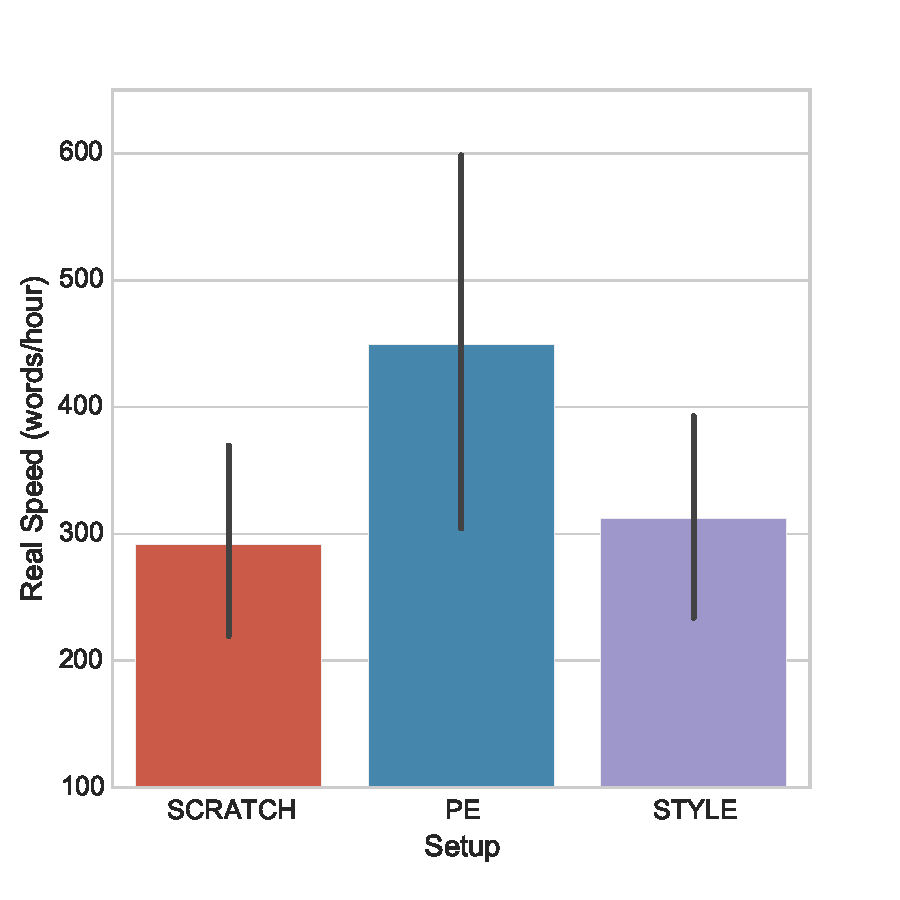
\includegraphics[width=0.45\textwidth]{img/time/time_real_setup}}
\subfloat[Text]{
\label{fig:time_real_text}
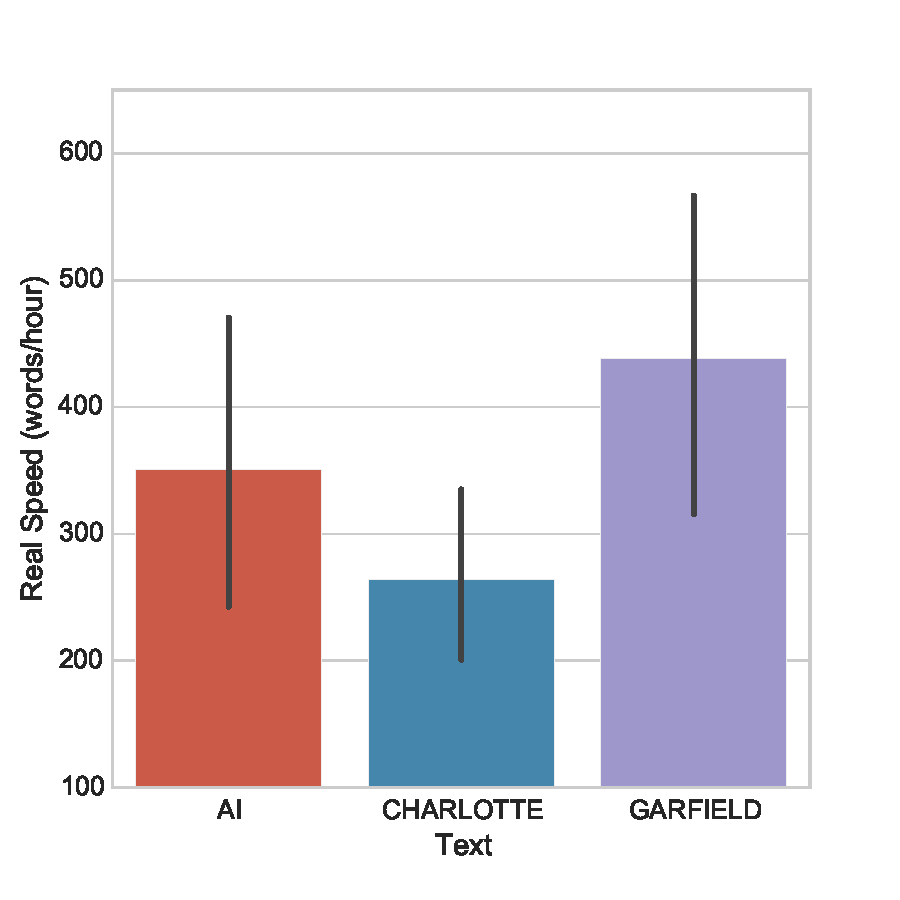
\includegraphics[width=0.45\textwidth]{img/time/time_real_text}}
\caption{Mean speeds per setup and per text. 95\,\% confidence interval calculated using bootstrap resampling.}
\label{fig:time_real_vs}
\end{figure}

\begin{figure}[h]
\myfloatalign
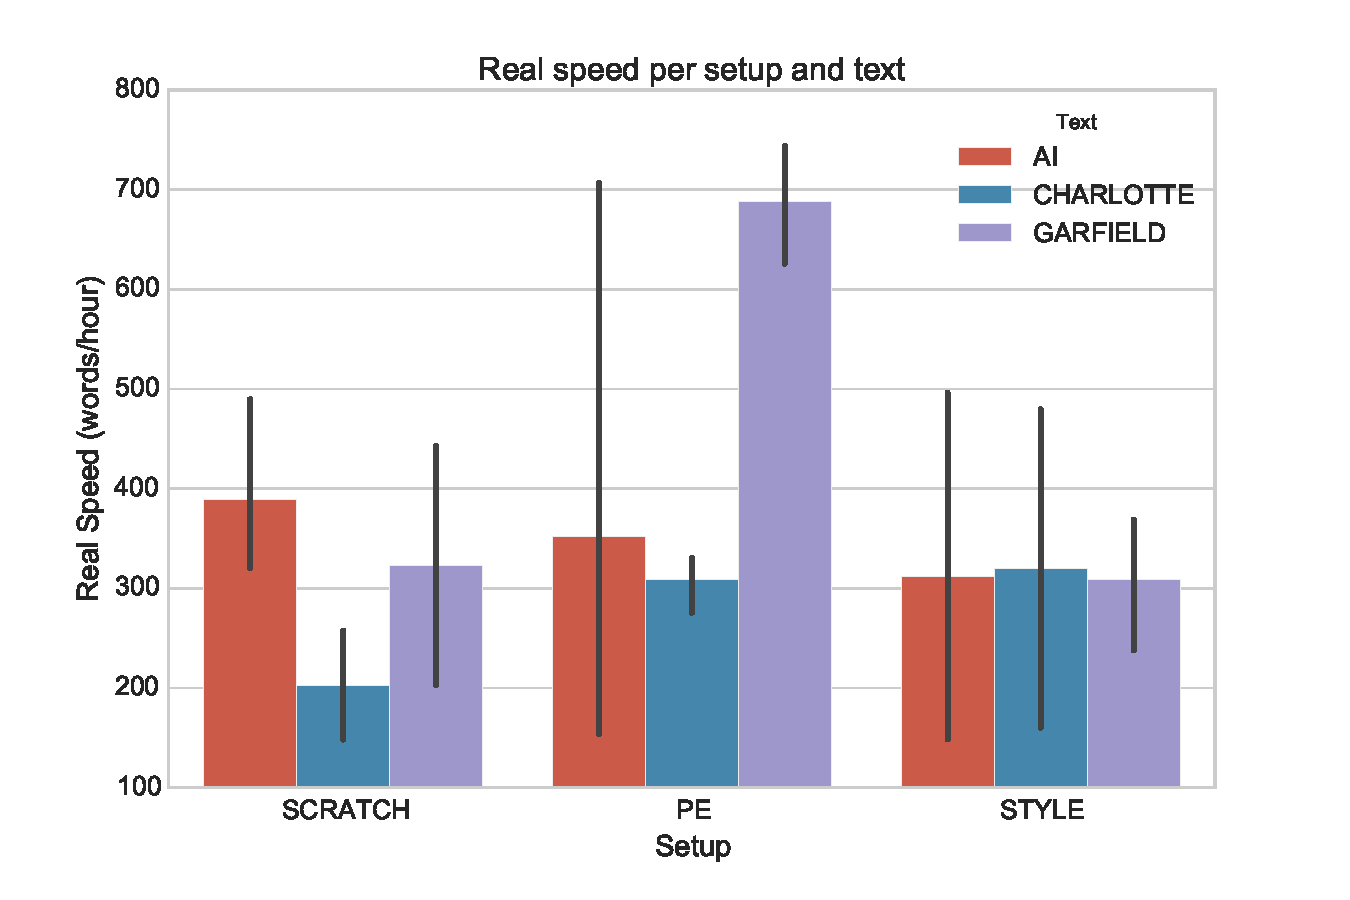
\includegraphics[width=0.8\textwidth]{img/time/time_real_ts}
\caption{Mean speeds broken down per setup and per text. 95\,\% confidence interval calculated using bootstrap resampling.}
\label{fig:time_real_ts}
\end{figure}

\subsection{Participants}

\noindent Individual variation is a strong factor in speed considerations. As can be seen in \autoref{fig:time_box_participant} and \autoref{fig:time_speed_participant}, speeds can range between just over 100 to over 700 $words/hour$ depending on the translator and the setup. Some participants such as 421, 423, 425 and 427 translate at a fairly constant speed across texts and setups. Others, such as 424 and 429, experience major speed differences across setups. In particular, \autoref{fig:time_speed_participant} shows these latter two participants experience a major speed-up in the \ac{PE} setup, which could indicate they only minimally edited the \ac{MT} output. To confirm this, \spacedlowsmallcaps{BLEU} \parencite{papineni2001bleu} scores were calculated between the \ac{MT} suggestions and the final post-edited translations. \spacedlowsmallcaps{BLEU} is usually used to score how well a machine-translated text matches a reference translation, here the metric is used to see how much editing was performed on the \ac{MT} suggestions by the participants. \autoref{fig:time_real_bleu} shows a correlation (Pearson's $r = 0.75$) between the \spacedlowsmallcaps{BLEU} scores and the time spent post-editing. This correlation is also present in the time participants thought they had spent on the task (\autoref{fig:time_perceived_bleu}, Pearson's $r = 0.8$).

\begin{figure}
    \myfloatalign
    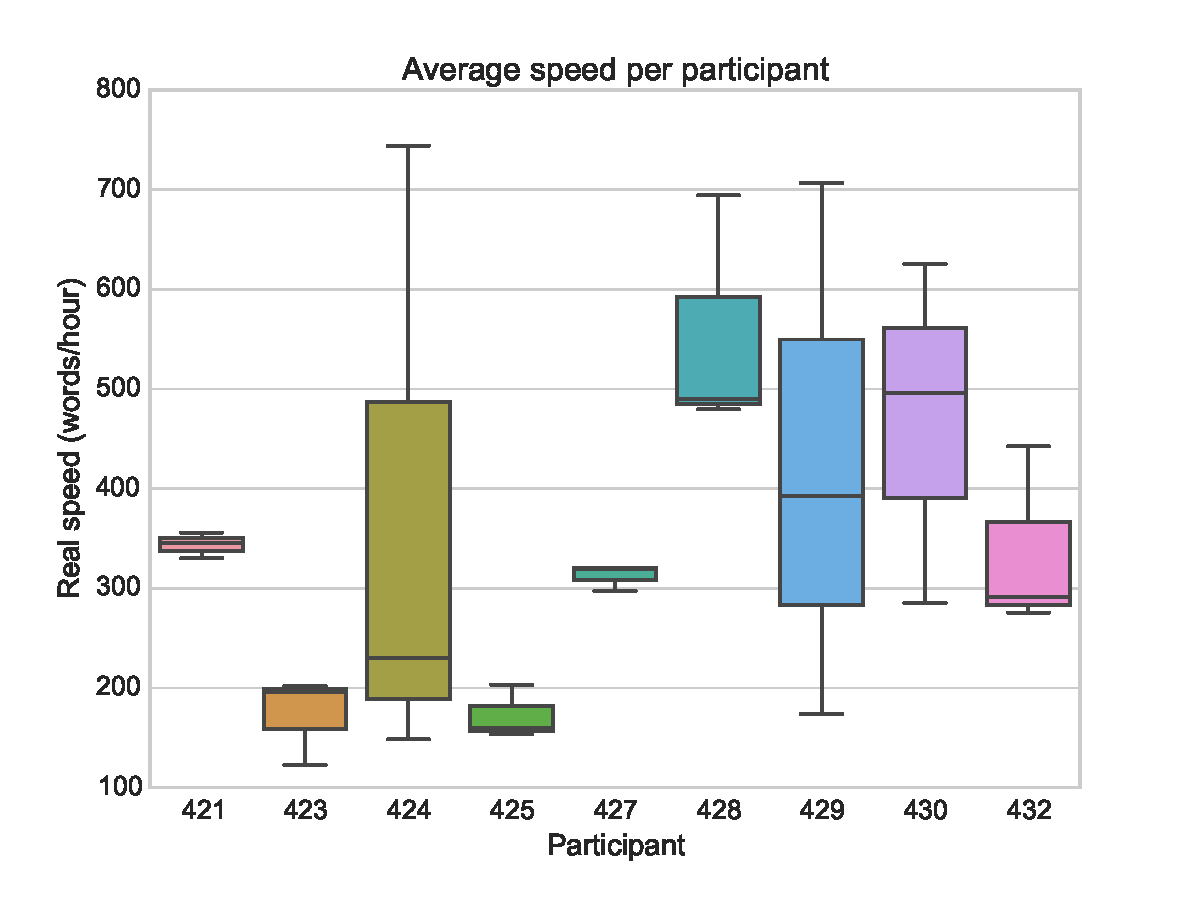
\includegraphics[width=0.8\textwidth]{img/time/time_box_participant}
    \caption{Mean real speeds per participant}
    \label{fig:time_box_participant}
\end{figure}

\begin{figure}
    \myfloatalign
    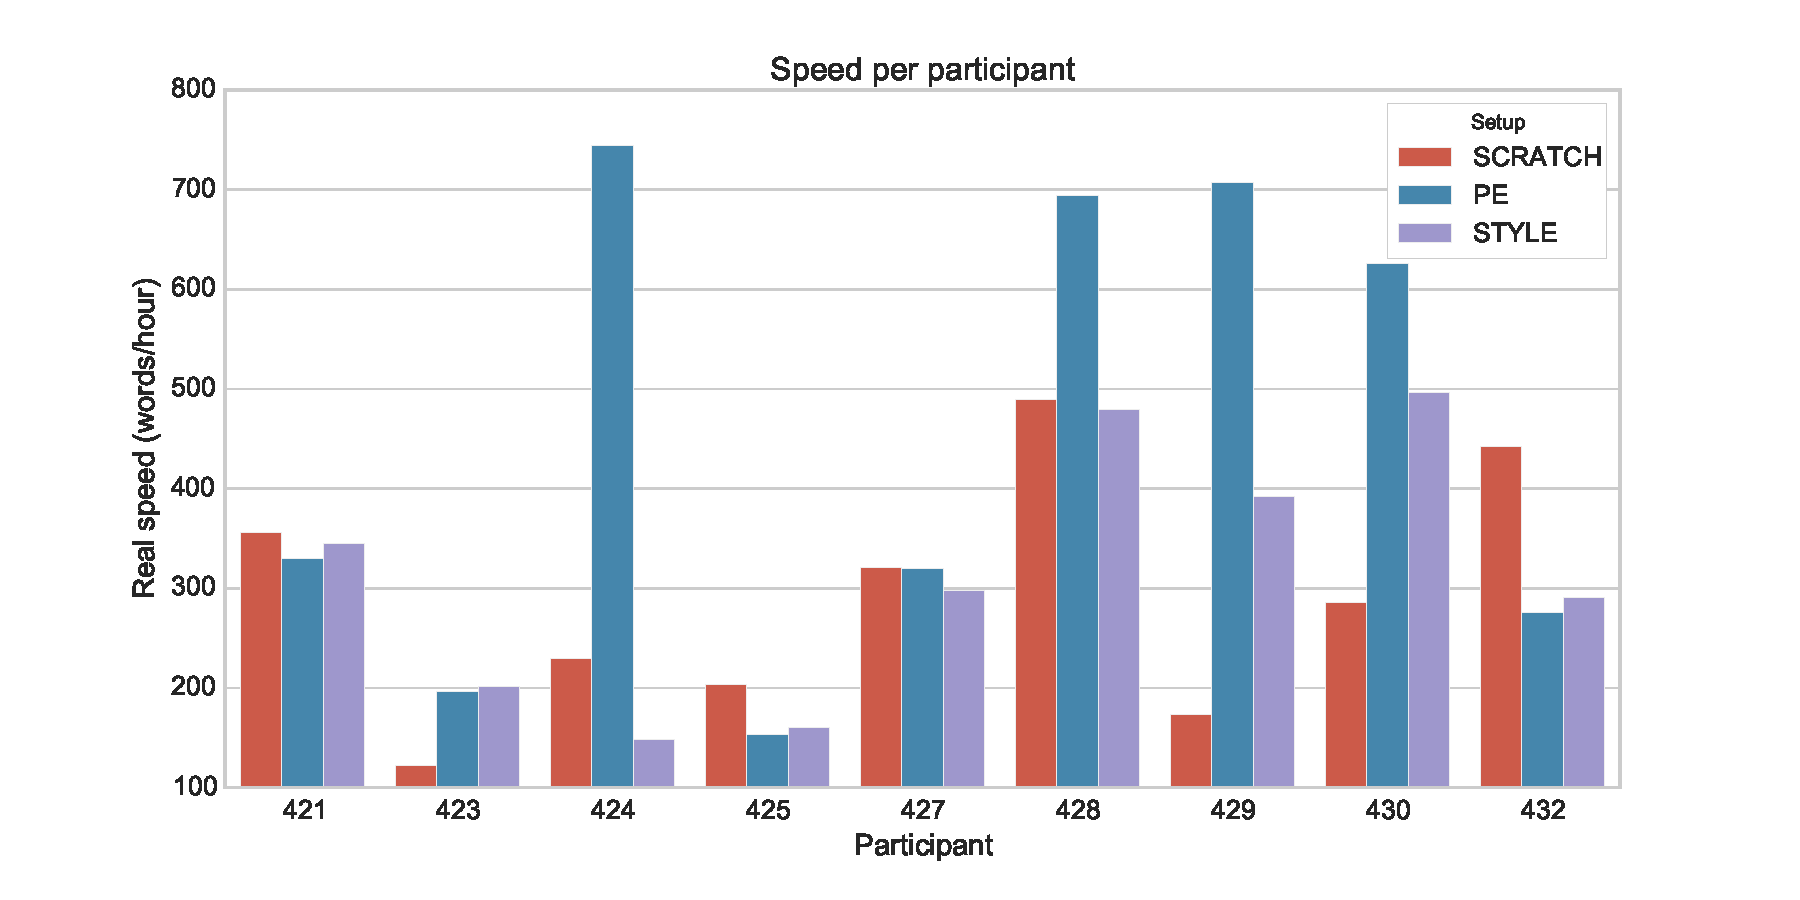
\includegraphics[width=\textwidth]{img/time/time_speed_participant}
    \caption{Real speed per participant and setup}
    \label{fig:time_speed_participant}
\end{figure}

\begin{figure}[H]
    \myfloatalign
    \subfloat[Real speed]{
        \label{fig:time_real_bleu}
    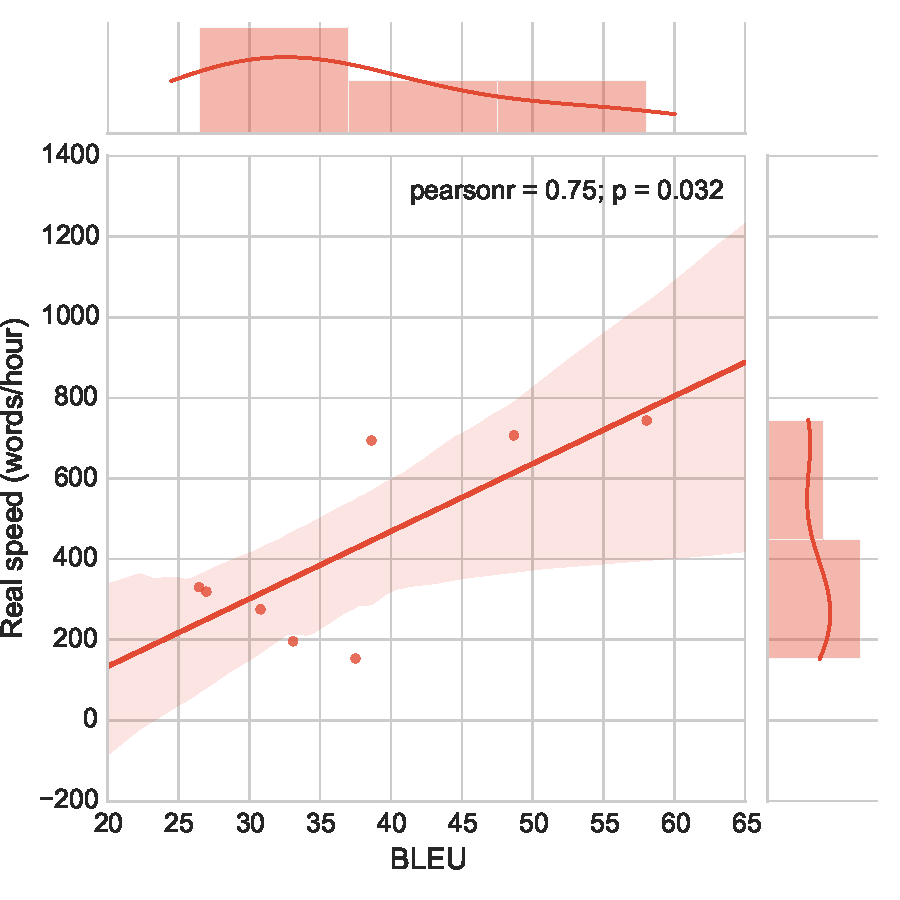
\includegraphics[width=0.45\textwidth]{img/time/time_real_bleu}}
    \subfloat[Perceived speed]{
        \label{fig:time_perceived_bleu}
    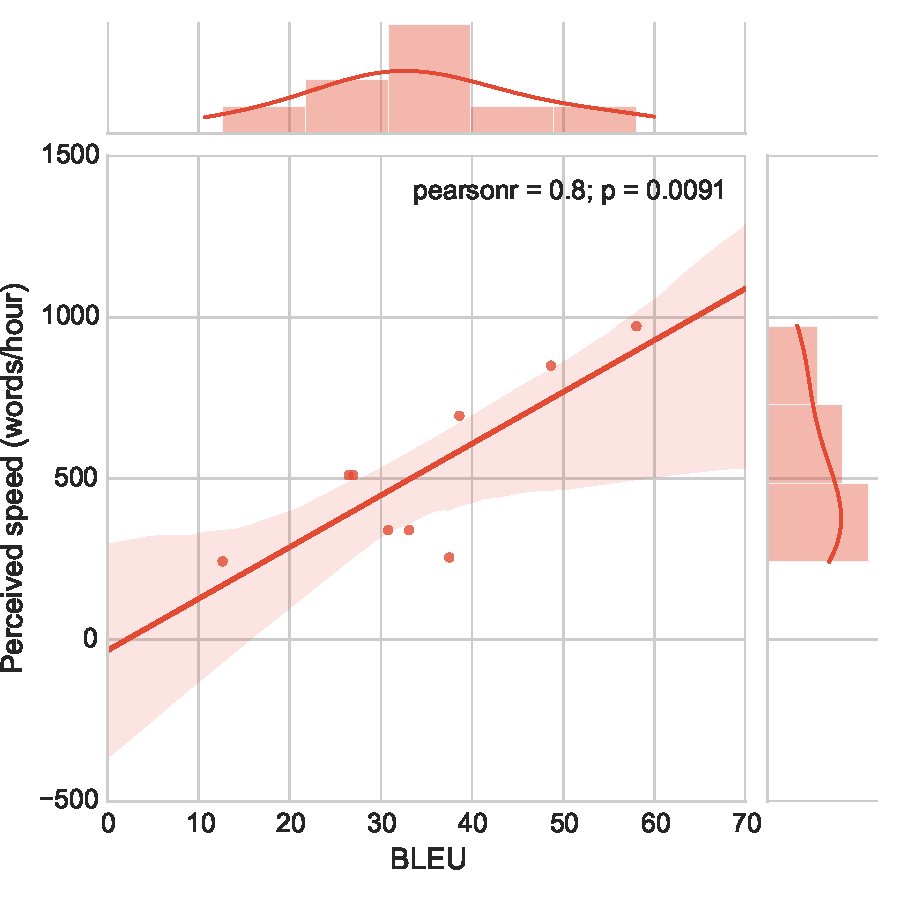
\includegraphics[width=0.45\textwidth]{img/time/time_perceived_bleu}}
    \caption{Correlation between real and perceived speed spent on post-editing and the final translation's \spacedlowsmallcaps{BLEU} score. Data from one participant was omitted from the real time as it was a clear outlier (including it, the correlation was $r = 0.39$)}
    \label{fig:time_bleu}
\end{figure}

Thus, it seems that the \ac{PE} only acheives an increase in speed when translators minimally edit the \ac{MT} suggestion. Participants were not given guidelines on how to use the \ac{MT} suggestions, so they were free to take the approach they preferred. If they feel they need to change the suggestion more, speed differences are negligible or can even result in a slow-down (\autoref{fig:time_diff_bleu}).

\begin{figure}[H]
\myfloatalign
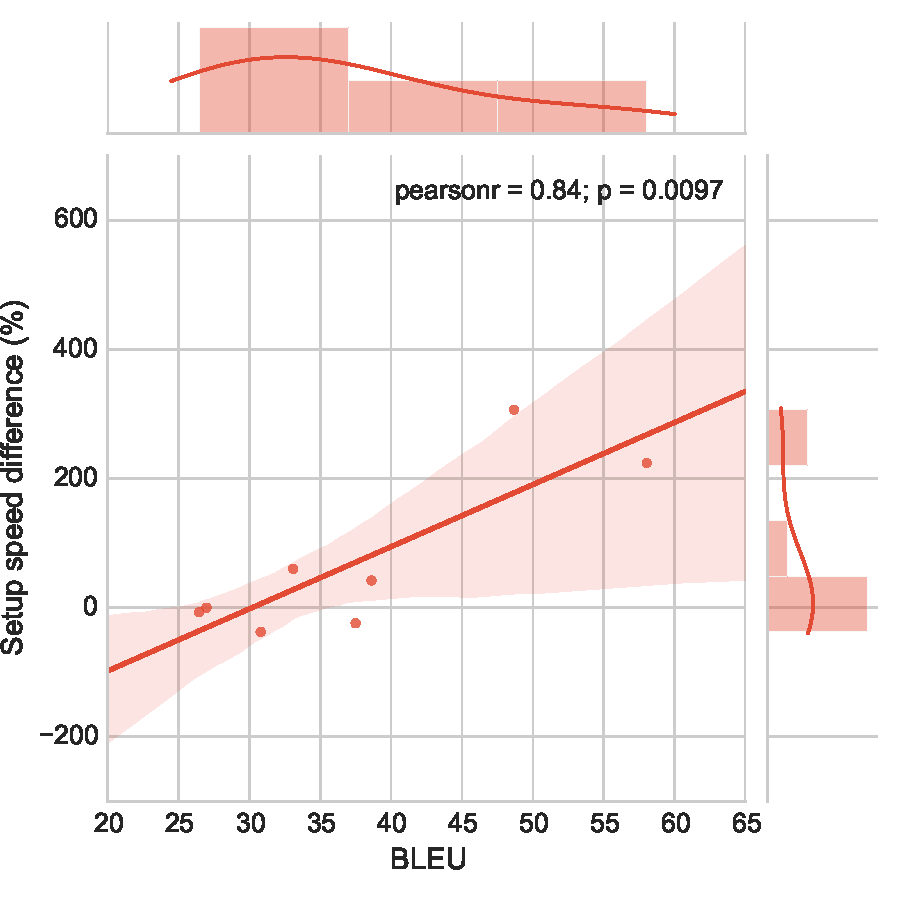
\includegraphics[width=0.5\textwidth]{img/time/time_diff_bleu}
\caption{Correlation between the \% speed difference between \scratch and \ac{PE} (positive indicates \ac{PE} was faster) and the final translation's \spacedlowsmallcaps{BLEU} scores. Data from one participant was omitted from the real speed as it was a clear outlier (including it, the correlation was $r = 0.56$)}
\label{fig:time_diff_bleu}
\end{figure}

\subsection{Perceptions of Time}

\noindent Perceived speeds have not been studied in previous literature on translation process research, thus there is no background in how to interpret them. I suggest they could also be considered a measure of effort. A tedious task raises awareness of the time being spent on it and makes people think they're spending more time on it than they actually have, while an easy and enjoyable task can seem faster. The results in this study seem to support this view. 

As can be seen in \autoref{fig:time_overall}, overall the translators thought they translated much faster than they actually did. Digging further into the data, \autoref{fig:time_real_vs_perceived} shows that participants felt that their speed between setups was roughly similar, with \ac{PE} as fastest and \style as slowest. This contrasts with the real speeds, which were roughly the same for \style and \scratch and faster for \ac{PE}.

In other words, participants were fairly accurate at predicting their time spent in \ac{PE}, but they felt \scratch and \style were faster than they actually were. This indicates that they were more aware of the time during \ac{PE}. Supposing a link between time awareness and effort, this would indicate \ac{PE} required more effort and was liked less.

\begin{figure}[h]
\myfloatalign
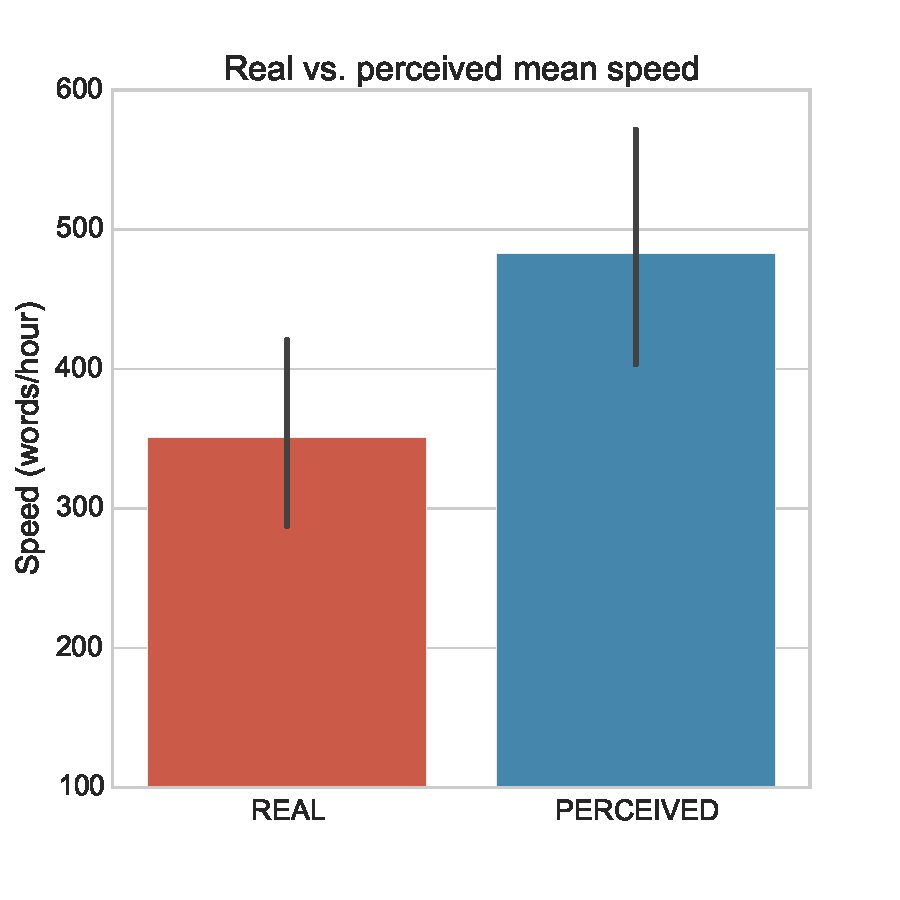
\includegraphics[width=0.5\textwidth]{img/time/time_overall}
\caption{Overall real vs. perceived mean speed. 95\,\% confidence interval calculated using bootstrap resampling.}
\label{fig:time_overall}
\end{figure}

As will be discussed in \autoref{sec:setup_prefs}, participants associated like and dislike more strongly with a particular text than with a particular setup. Looking at the speed per text in \autoref{fig:time_real_vs_perceived}, we see participants perceived \charlotte as being the slowest text to translate, which lines up with it being considered the hardest (\autoref{sub:like_dislike}). \ai was both considered the hardest (4 participants) and the second easiest (3 participants), which could explain why its average perceived speed is roughly as fast as \spacedlowsmallcaps{garfield}, which is considered the easiest translation (5 participants). 

\begin{figure}
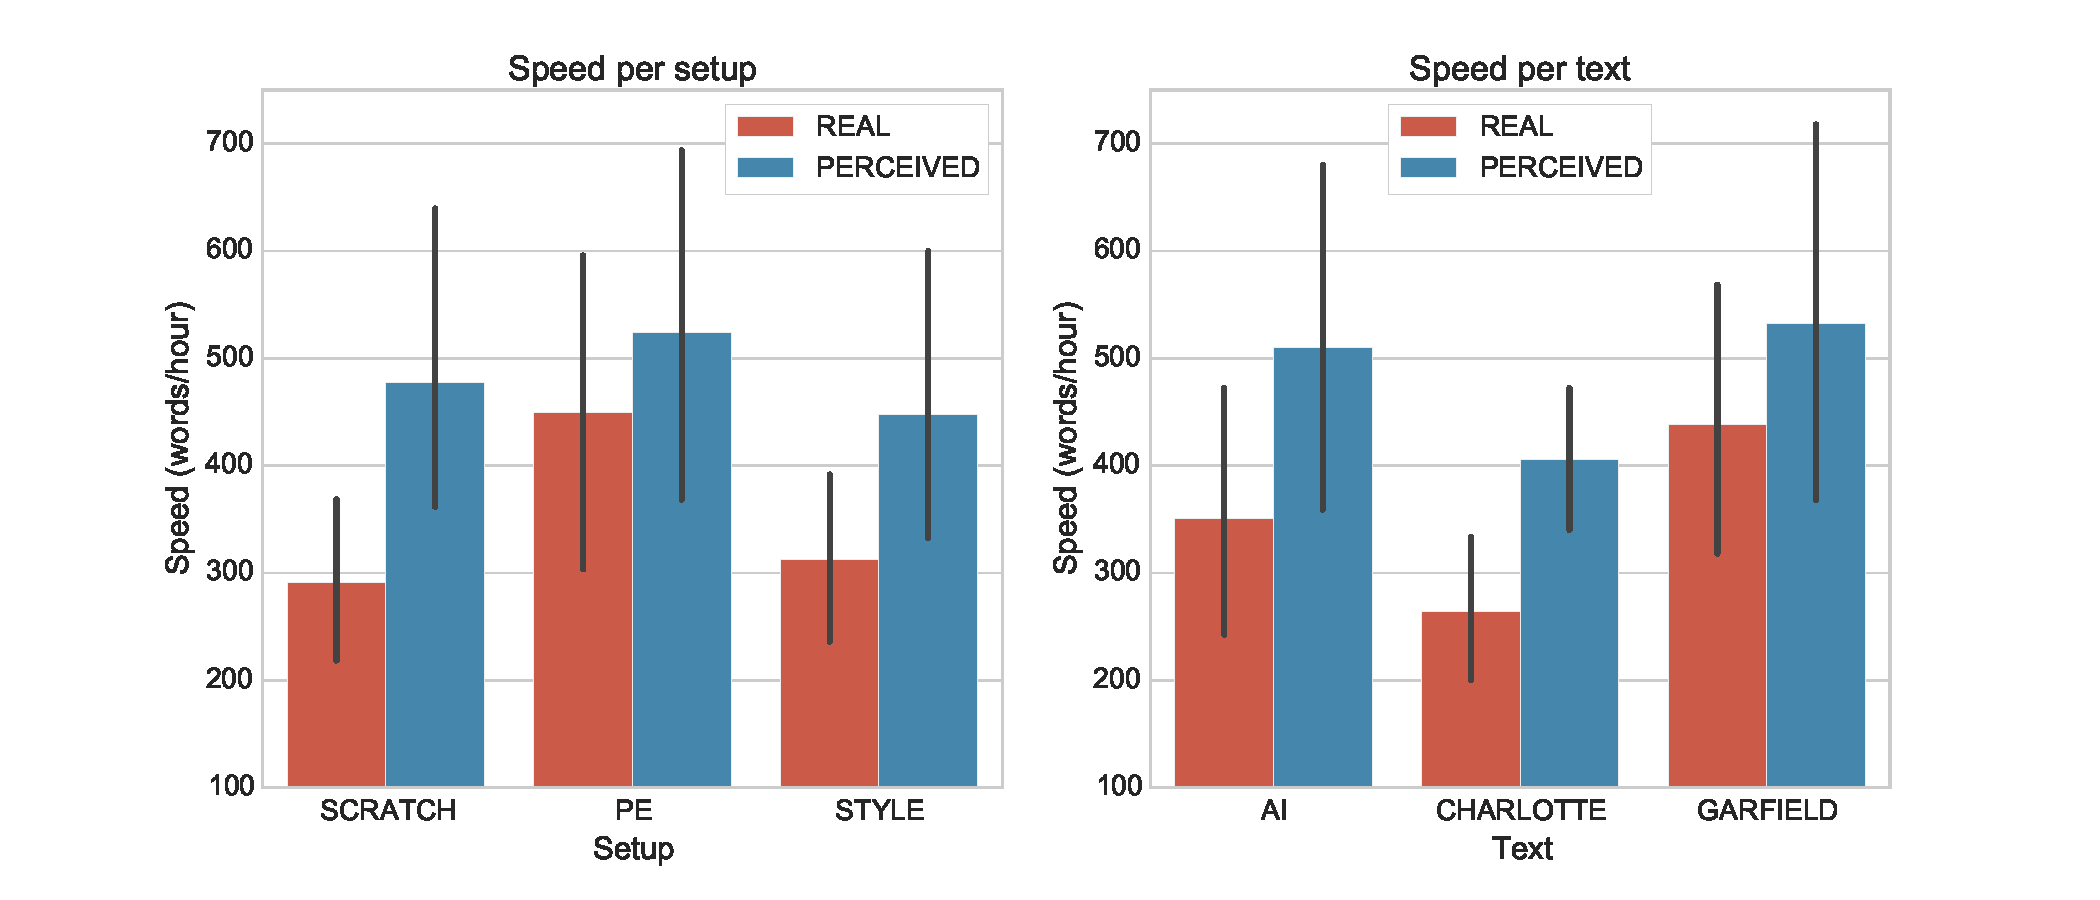
\includegraphics[width=\textwidth]{img/time/time_real_vs_perceived}
\caption{Real vs. perceived speed per setup and per text. 95\,\% confidence interval calculated using bootstrap resampling.}
\label{fig:time_real_vs_perceived}
\end{figure}

%----------------------------------------------------------------------------------------

\section{Setup Preferences}
\label{sec:setup_prefs}

\noindent In order to determine which setup the participants preferred, two key questions were asked: whether they would have preferred to translate from scratch without the \ac{MT} suggestion and without the StyleCheck hints [Questions 21 and 31]. 44\,\% said they would prefer not to have the \ac{MT} suggestions versus 33\,\% who would prefer not to have the StyleCheck suggestions. Thus, overall acceptance is higher for StyleCheck than for \ac{PE}. The acceptability rate for \ac{PE} was higher among this study's participants than in other studies such as in \textcite{carl2015post}, where 83\,\% of participants responded preferring translating from scratch. \textcite{carl2015post} does report a higher satisfaction rate for the \ac{PE} task among students versus professionals. Since this study's participants had limited experience as translators ($<2$ years), they could be considered closer to the student category than the professional category. This could explain the higher acceptability rate.

\subsection{Satisfaction}

\noindent Participants were asked to rate their satisfaction both for the task and the quality of their final translation for each setup [Questions F.14-15, F.22-23, F.32-33]. Task satisfaction results in \autoref{tab:satisfaction} indicate that \ac{PE} was the most satisfactory setup, followed by \scratch and \style in final place. Quality satisfaction results (\autoref{tab:satisfaction}) indicate a similar trend, with \ac{PE} providing the highest quality satisfaction, followed by \style and then \spacedlowsmallcaps{scratch}. These results seem to be in direct opposition to those discussed in the previous paragraph, where the majority of participants preferred the \scratch setup, followed by \style and \ac{PE}. It should be noted, however, that the means are always between 1 and 3, indicating participants were not dissatisfied with any of the setups or resulting quality.

\begin{table}[h]
    \subfloat[Task satisfaction]{
        \label{tab:sat_task}
        \begin{tabularx}{0.45\textwidth}{Xcc}
            \toprule
            \tableheadline{Setup} & \tableheadline{Mean rating} & \tableheadline{\sigma} \\
            \midrule
            \scratch &  $2.2$ & $0.4$\\
            \ac{PE} &  $1.9$ & $0.6$ \\
            \style &  $2.4$ & $0.9$ \\
            \bottomrule
    \end{tabularx}}
    \quad
    \subfloat[Quality satisfaction]{
        \label{tab:sat_quality}
        \begin{tabularx}{0.45\textwidth}{Xcc}
            \toprule
            \tableheadline{Setup} & \tableheadline{Mean rating} & \tableheadline{\sigma} \\
            \midrule
            \scratch &  $2.7$ & $0.9$\\
            \ac{PE} &  $1.9$ & $0.8$ \\
            \style &  $2.4$ & $1.2$ \\
            \bottomrule
    \end{tabularx}}
    \caption{Mean ratings and standard satisfaction ratings with the task and the final translation quality broken down by setup. Ratings range from 1 (Very satisfied) to 5 (Very dissatisfied).}  
    \label{tab:satisfaction}
\end{table}

\begin{table}[h]
    \subfloat[Task satisfaction]{
        \label{tab:sat_task_text}
        \begin{tabularx}{0.45\textwidth}{Xcc}
            \toprule
            \tableheadline{Text} & \tableheadline{Mean rating} & \tableheadline{\sigma} \\
            \midrule
            \ai &  $2.4$ & $0.7$\\
            \charlotte &  $2.4$ & $0.7$ \\
            \garfield &  $1.9$ & $0.6$ \\
            \bottomrule
    \end{tabularx}}
    \quad
    \subfloat[Quality satisfaction]{
        \label{tab:sat_quality_text}
        \begin{tabularx}{0.45\textwidth}{Xcc}
            \toprule
            \tableheadline{Text} & \tableheadline{Mean rating} & \tableheadline{\sigma} \\
            \midrule
            \ai &  $2.7$ & $0.9$\\
            \charlotte &  $2.4$ & $1.0$ \\
            \garfield &  $1.9$ & $1.1$ \\
            \bottomrule
    \end{tabularx}}
    \caption{Mean ratings and standard deviation for satisfaction ratings with the task and the final translation quality broken down by text. Ratings range from 1 (Very satisfied) to 5 (Very dissatisfied).}  
    \label{tab:satisfaction_text}
\end{table}

We hypothesise that the result disparity just described is due to participants linking satisfaction more strongly to the texts that were translated rather than the setups they were translated in. \autoref{tab:satisfaction_text} shows the results of braking the satisfaction down by text. \garfield always comes out top, which is in line with it being the most liked text (\autoref{sub:like_dislike}). A larger participant pool would be required to obstain more conclusive results.

\subsection{Like/Dislike, Easy/Difficult and Control}
\label{sub:like_dislike}

\noindent To provide more context to the satisfaction ratings, participants were asked what they liked or disliked about the setups [Questions F.12-13, F.18-19, F.26-27]. They were also asked what translations where the hardest and the easiest [Questions F.3-6] and during which setups they felt they had the most and least control [Questions F.7-10]. We discuss each of these separately.

The majority of participants mentioned textual considerations as a factor in deciding whether a text was easy or hard [Questions F.3-6]. These included text structure, topic, terminology, etc. When asked why a text/setup was hard, one participant complained that editing the \ac{MT} suggestion doubled the amount of work compared to translating from scratch. When asked why they had chosen a text/setup as the easiest, two participants mentioned that post-editing an \ac{MT} suggestion was faster and easier. When braking down the results by text, \garfield is mentioned as the easiest (56\,\% of participants) and is the chosen the least times as the most difficult (only one participant). \charlotte turns out to be the most difficult if we combine that it's in joint first place for the most difficult (\ai and \charlotte have 4 counts each) and it receives just a single count as the easiest.

The case of the AI is interesting. Considered both the hardest (4 participants) and the second easiest (3 participants) to translate, the data shows no correlation between its hard/easy consideration and having translated it in a particular setup. This further strengthens the view that difficulty is linked to a certain text rather than a certain setup, although as previously mentioned setups can play a part in this.

As for what was liked or disliked, participants mentioned more frequently in their open answers aspects relating to the text topic or specific textual elements. Specifically, \garfield seems to have been the text most liked by participants. The quality and usefulness of the \ac{MT} suggestions also appear fairly frequently. Once again, it seems that the texts have more of an influence on what participants liked or disliked than specific. 

Finally, the data on control or lack of it paints a similar picture. When asked where they felt they had the most control [Question F.7-8], responses were spread equally among setups but showed great variation in texts: \garfield made them feel most in control, followed by \ai and \charlotte. Open answers present as reasons a mix of textual considerations (participants knew a lot about Garfield, there were no tricky terms) and setup considerations (some disliked have suggestions or hints of any kind). As for where they had least control [Questions F.9-10], results again show a flat variation among setups but differences in texts: \ai made them feel the least in control, followed by \charlotte and \garfield. Here, the open answers overwhelmingly mention textual considerations such as the topic and terminology.

\subsection{Causes}

\noindent To throw further light onto the high acceptance of the \ac{PE} setup, we can look at the quality ratings for the \ac{MT} suggestions. Following \textcite{carl2015post} and what is commonplace in \ac{MT} evaluation, participants were asked to rate the \ac{MT} quality on three criteria: grammaticality, style and accuracy [Question F.20]. Results (\autoref{tab:mt_eval}) show all three criteria were considered average, edging towards above average. There were even some counts of well above average grammaticality (1 count) and style (1 count). This in contrast to participants in \textcite{carl2015post}, who rated all criteria closer to below or well below average. A perceived higher quality of the \ac{MT} suggestions explain the higher acceptance of \ac{PE} in this study. As for the \style setup, further discussion is provided in \autoref{sec:sc_effectiveness}.

\begin{table}[h]
\myfloatalign
\begin{tabularx}{0.5\textwidth}{Xcc}
\toprule
\tableheadline{Criteria} & \tableheadline{Mean rating} & \tableheadline{\sigma} \\
\midrule
Grammaticality &  $2.7$ & $1.0$\\
Style &  $2.6$ & $0.7$ \\
Accuracy &  $3.0$ & $1.0$ \\
\bottomrule
\end{tabularx}
\caption{Mean ratings and standard deviation for \ac{MT} quality evalutaions. Ratings ranged from 1 (Well above average) to 5 (Well below average), with 3 being Average.}
\label{tab:mt_eval}
\end{table}

\subsection{Summary of Preferred Setups}

\noindent Thus, after the previous considerations, the data indicated that participants' preferred setup was \spacedlowsmallcaps{scratch}, followed by \style and \ac{PE}. This is essentially based on Questions F.21 and F.31.

The previous findings also make it is reasonable to suppose that participants perceive the specific text (topic and textual considerations) as having the most influence in their preferences and enjoyment of a translation (degree of easiness, like/dislike, and task and quality satisfaction). This is useful insight for designing questionnaires whose aim is to evaluate a tool. Although the free form answers do provide some insight into the tool, it is best evaluated with a direct question of the kind ```Whould you have preferred to translate without $X$?''.

%----------------------------------------------------------------------------------------

\section{StyleCheck Effectiveness}
\label{sec:sc_effectiveness}

\noindent This section evaluates the efectiveness of StyleCheck by analysing the actual translations produced by the participants. Before delving into the details, it is important to determine whether participants considered that sticking to the Wikipedia \ac{SG} rules was important (just as the translation brief stated it was).

\subsection{Style Guide Importance}

\noindent Participants were asked if they had established any priorities and restrictions after reading the brief and, if yes, which ones [Questions F.1 and F.2]. The notion of priorities and restrictions is taken from \textcite{zabalbeascoa1999priorities}, and describes the hierarchical list of aims and goals that translators establish for a translation after taking all factors into account (\ac{ST}, target culture, client requirements, deadline and even pay). 67\,\% reported having established priorities and restrictions. Out of these, half explicitly mentioned following the Wikipedia Style Guide as their top prority. One participant mentioned specific aspects of the writing style used in Wikipedia, and the rest mentioned general strategies of translation. Thus, the translation brief succeeded in making most participants prioritise style guide application. The others may have not prioritised it considering that the translations were short and they were not receiving compensation for the experiment, making it not worth the time and effort to read the whole style guide and follow it. This would also fit in with the model of priorities and restrictions, which as mentioned before allows for time and payment considerations to come into play.

Participants were asked if they had consulted the Wikipedia style guide linked in the brief [Question F.28]: 67\,\% said they had. Logging carried out on the server indicates the link to the Wikipedia Style Guide was only clicked by a third of the participants, one of which answered that they hadn't consulted the style guide. This could be due to participants opening up a new tab and searching for the style guide themselves, but given that the link was provided on all translation pages, this seems unlikely. It seems participants felt they should have consulted it, but preferred to say they had when they actually had not. This is a strong indicator of the usefulness of a digitally applied style guide: participants felt compelled to apply it, but did not. As stated before, this was probably due to the lack of time and short texts which did not make up for the investment in time required to read and apply the style guide.

When asked why [Question F.29], those who hadn't consulted the guide said they were not used to using style guides or that they had previously translated Wikipedia articles and were familiar with it. Those who had, either stated the general importance of using a style guide when one is provided by a client or mentioned specific elements they looked up (use of italics, parenthesis, how to handle names of works of art, etc.).

\subsection{Style Guide Application}

\noindent To evaluate how well StyleCheck worked, we first look at the objective data of whether a particular rule was applied or not in each translation. \autoref{fig:rules_1a} presents how many times the rules identified in the texts were applied or not. The \spacedlowsmallcaps{mixed} category refers to elements that appear more than once in a single text and present inconsistencies: some instances follow the associated style rule, others don't. The \spacedlowsmallcaps{avoided} category refers to instances where the text was changed, resulting in the rule issue being avoided. As can be seen, the \style setup leads to a notably higher amount of rules applied than the other setups. This is further confirmed in \autoref{fig:rules_1b}, which shows the data only for rules that were implemented in StyleCheck.

\begin{figure}[h]
\subfloat[Total rules]
{\label{fig:rules_1a}
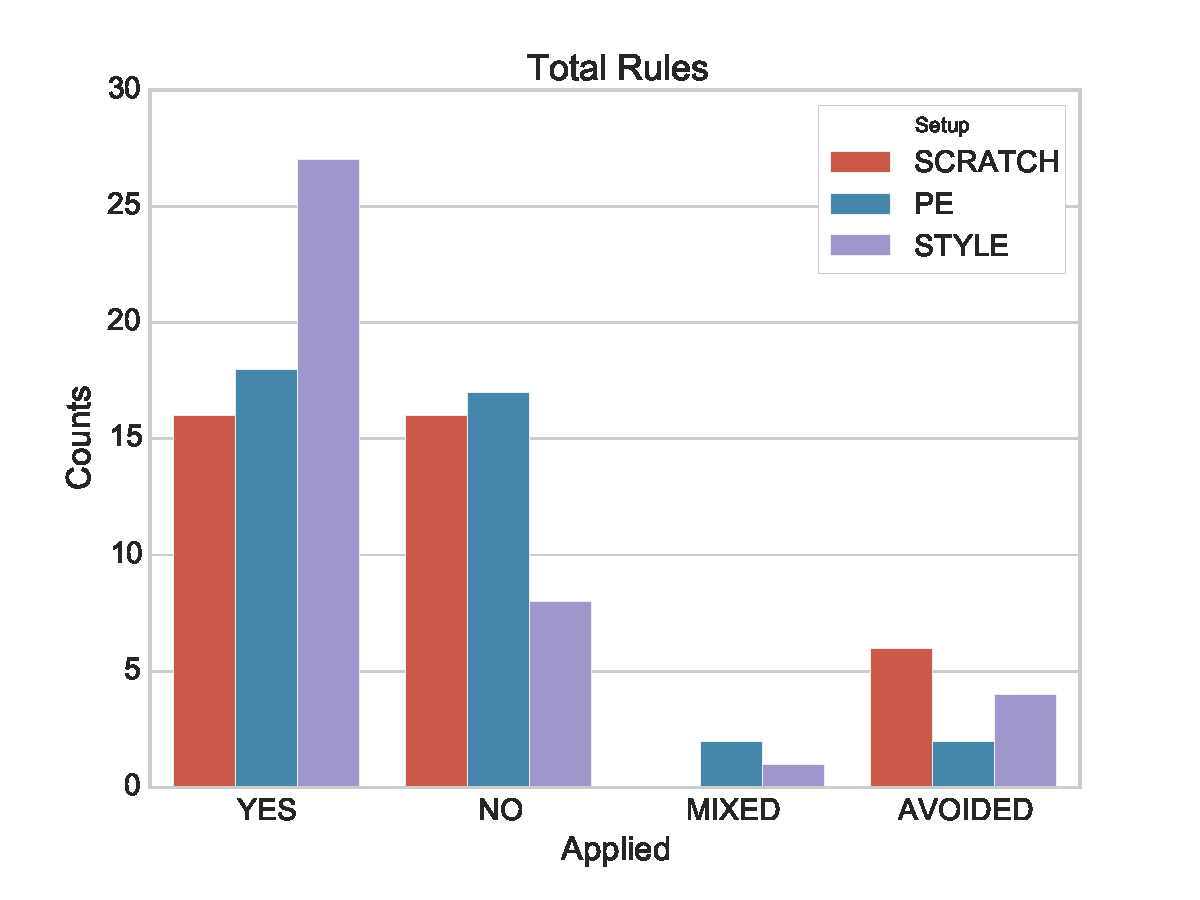
\includegraphics[width=0.5\textwidth]{img/rules/rules_1a}}
\subfloat[Rules implemented in StyleCheck]
{\label{fig:rules_1b}
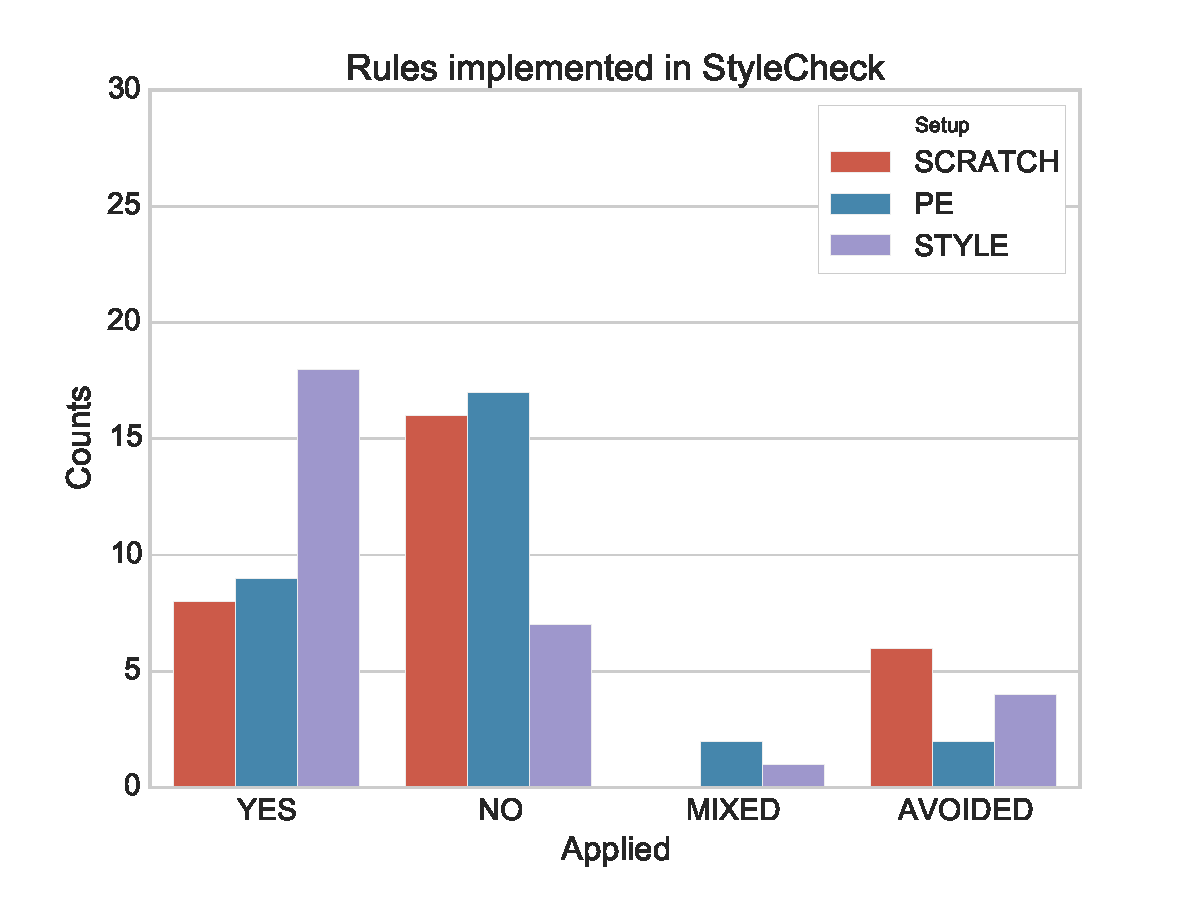
\includegraphics[width=0.5\textwidth]{img/rules/rules_1b}}
\caption{Number of rules that were applied in the final translations. Both the total number of rules detected in the texts and the subset of rules implemented in StyleCheck are presented.}
\label{fig:rules_1}
\end{figure}

Rule application varied a lot depending on the particular rule, as can be seen in \autoref{fig:rules_2}. Some rules, such as \spacedlowsmallcaps{3b} and \spacedlowsmallcaps{3c} were always applied. They were related to aspects (number formatting) that translators usually know are contained in style guides and may have previous experience in how to handle. Others, such as \spacedlowsmallcaps{2a} and \spacedlowsmallcaps{2b} were generally not applied. These were related to aspects very specific to the Wikipedia style guide (chronologiclly ordering lists and avoiding time expressions that refer to the moment of enunciation).

\begin{figure}[H]
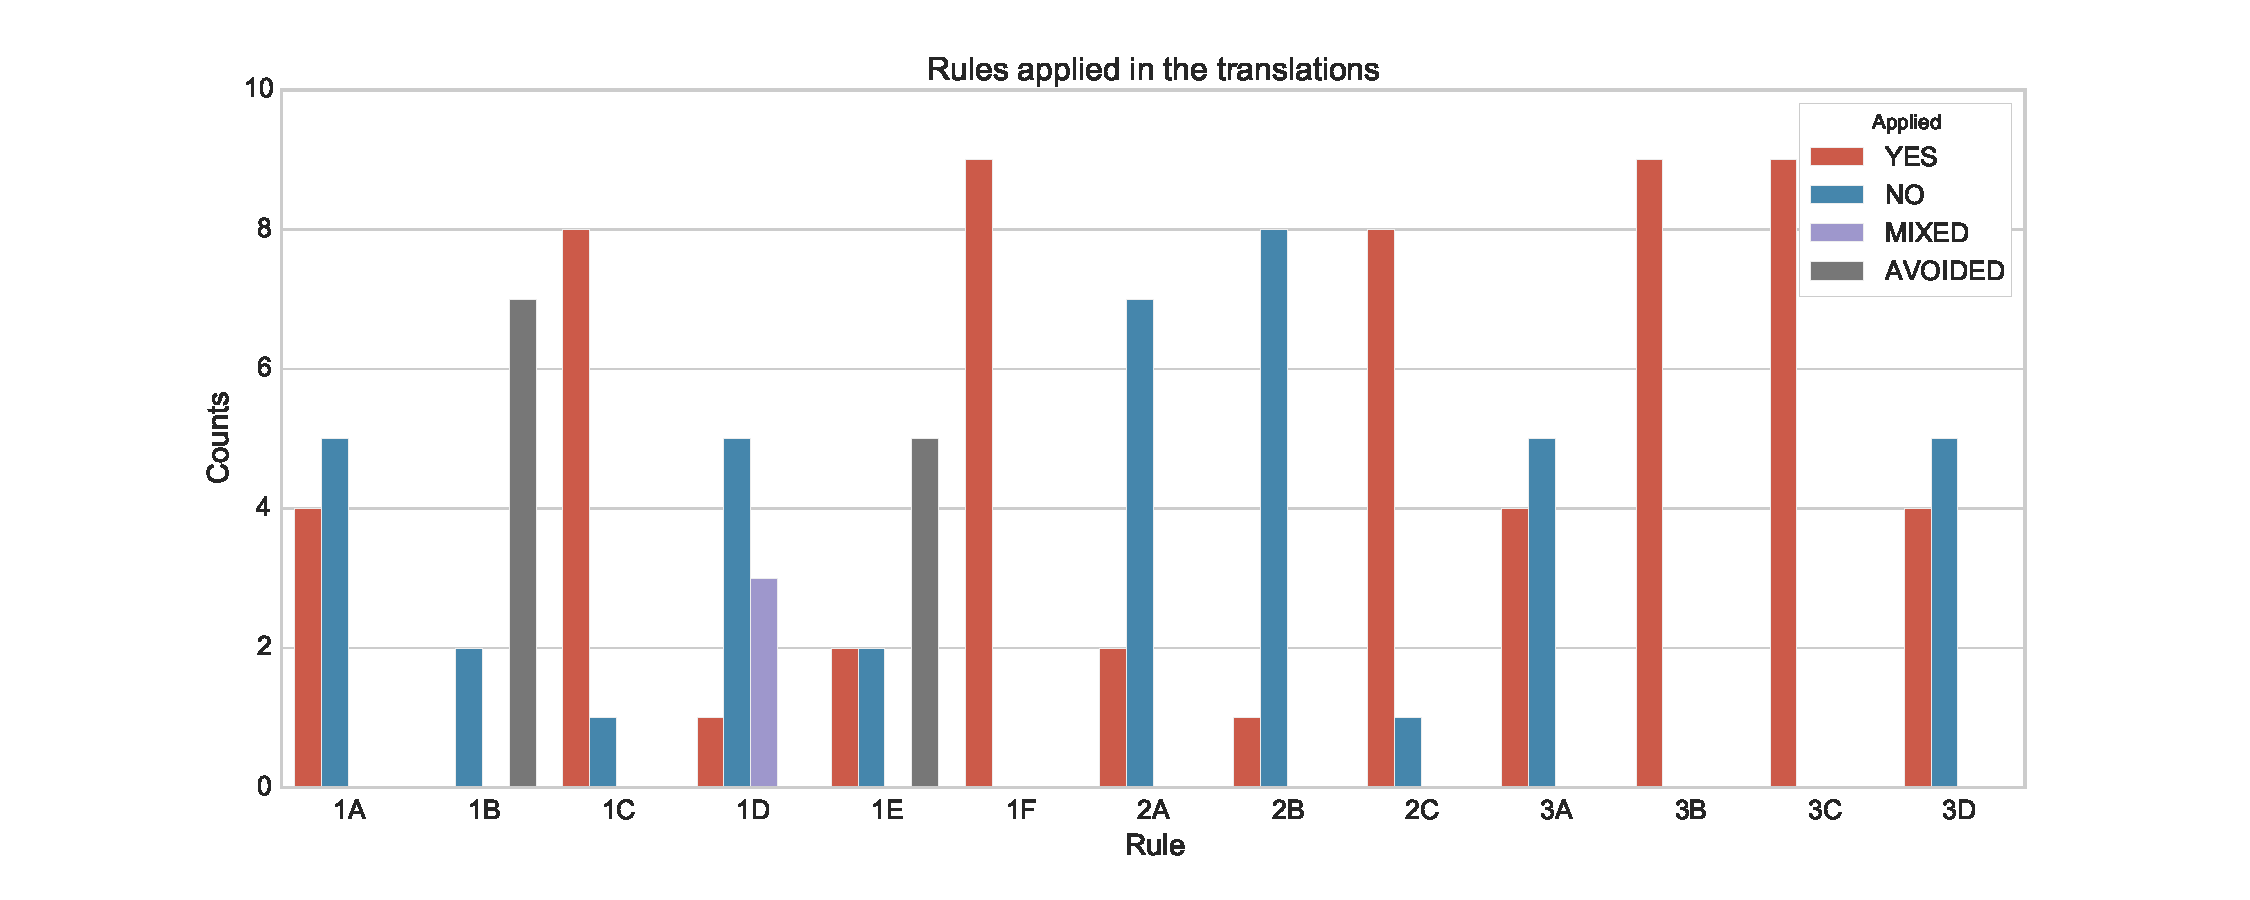
\includegraphics[width=\textwidth]{img/rules/rules_2}
\caption{Number of rules applied in the final translations for all setups. Counts are broken down by rule.}
\label{fig:rules_2}
\end{figure}

\subsection{StyleCheck vs. \ac{PE}}

\noindent We now turn to a comparison of the \style and \ac{PE} setups. Starting off with \ac{PE}, we find that participants tended to closely follow what the \ac{MT} suggestion presented. \autoref{fig:rules_3a} shows that all instances of rules that were applied in the \ac{MT} suggestion were also applied in the final translation. \autoref{fig:rules_3b} shows similar results: 67\,\% of rules not applied in the suggestion were not applied in the final translation. Only 25\,\% of them were corrected so that they were correctly applied. The mixed instances in the \ac{MT} suggestion provide further evidence: two out of the three instances were also carried on to the final translation. With a simple revision of the final translation, participants should have noticed the inconsistencies and homogenised them.

\begin{figure}[H]
\myfloatalign
\subfloat[Rules applied in \ac{MT}]
{\label{fig:rules_3a}
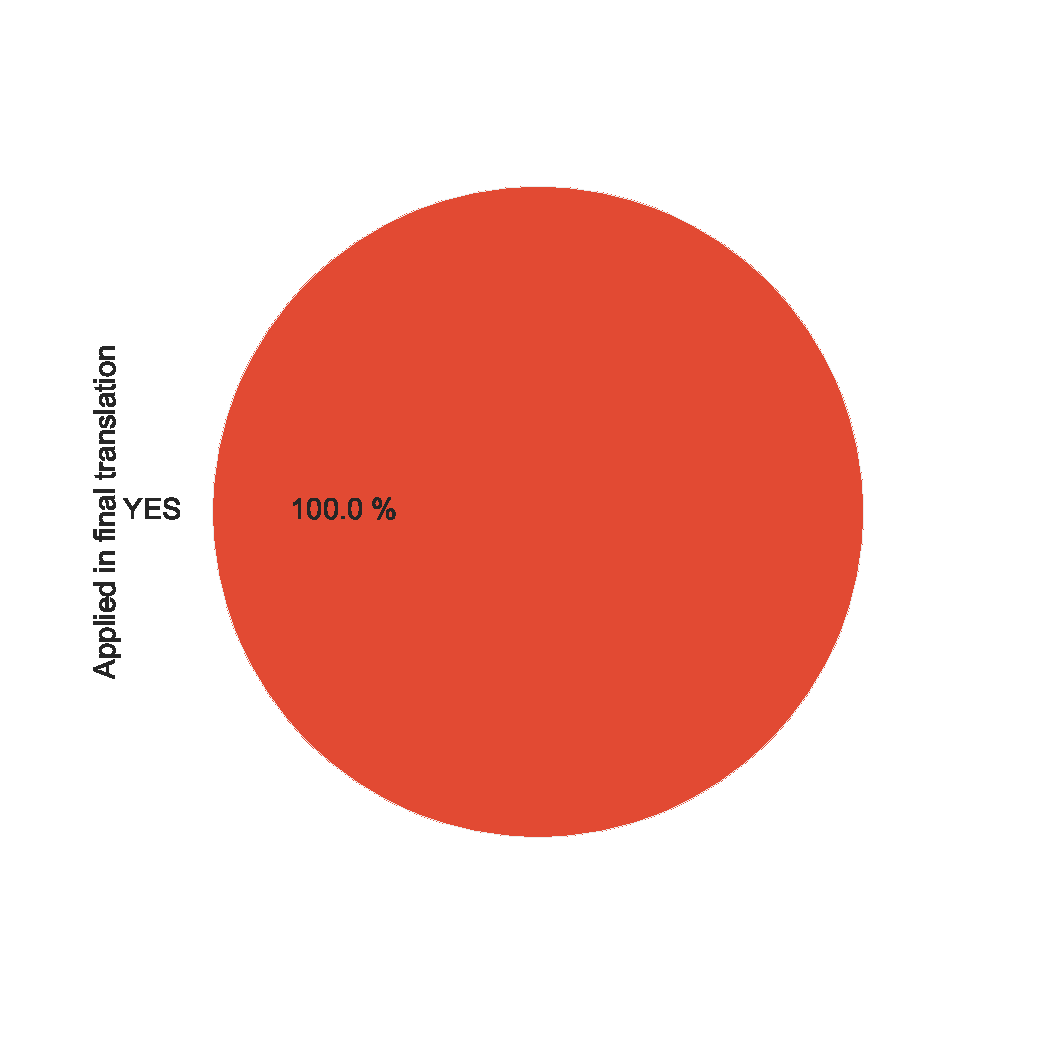
\includegraphics[width=.45\linewidth]{img/rules/rules_3a}}
\subfloat[Rules not applied in \ac{MT}]
{\label{fig:rules_3b}
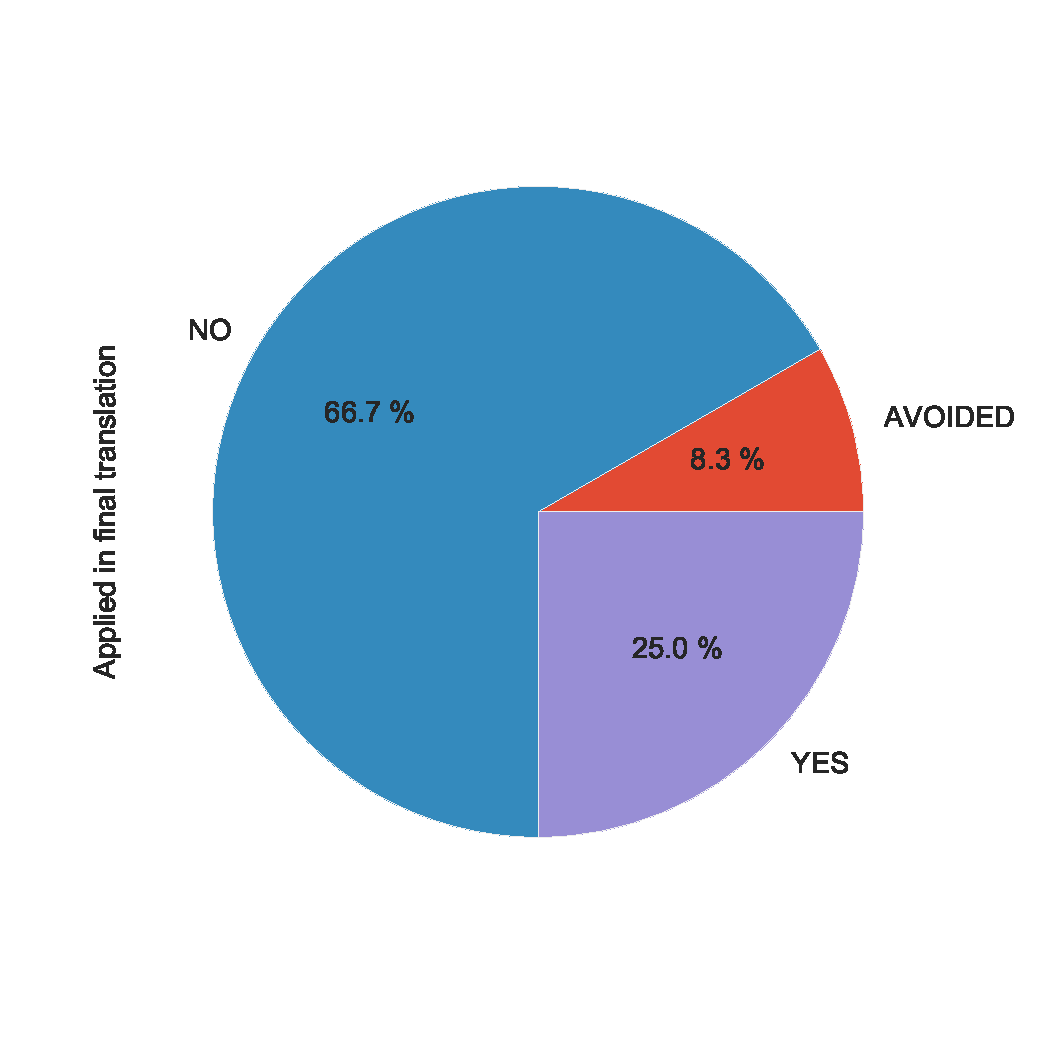
\includegraphics[width=0.45\linewidth]{img/rules/rules_3b}}
\caption{Percentage of rules applied or not in the final translation for the \ac{PE} setup depending on whether the\ac{MT} suggestion had applied them or not.}
\label{fig:rules_3}
\end{figure}

Delving further in the data, we find that StyleCheck was effective in getting participants to follow the suggestions. When presented with a suggestion (indicating the participant had written a sentence that did not follow a specific rule), 71\,\% of the time participants corrected their translations so that they followed the suggestion. 

To find out why in 29\,\% of the cases the suggestions weren't followed, we can check two sources of data, objective and subjective. Objective data indicates that out of the five cases where the suggestion wasn't followed, in two cases the relevant suggestion was shown in third position below two other suggestions. It is possible that depending on the screen resolution and browser window configuration the suggestion appeared outside of the screen and was not seen or ignored. The fact that some suggestions were long could have also contributed to this. A further two cases presented the suggestion in first position, indicating the participant ignored the suggestion or chose not to follow it. 

Subjective data was collected through the final questionnaire [Question F.30] and is presented in \autoref{tab:sc_eval}. Participants rated their agreement with various satements from 1 to 5. Participants generally agreed that the style hints were helpful, and agreed that the information they contained was right. Results show participants generally thought the style hints were easy to understand, but tended to agree that they were too long. This would suggest the hints could be improved by rewriting them into a tenser alert style, rather than copy the original style guide description. Regarding the user interface, participants on average remained rather neutral on whether there were too many hints and whether the boxes were distracting. However, both considerations included one instance of a participant strongly agreeing.


\begin{table}[h]
\myfloatalign
\begin{tabularx}{\textwidth}{Xcc} \toprule
\tableheadline{Consideration} & \tableheadline{Mean agreement} & \tableheadline{\sigma} \\
\midrule
The style hints were helpful & $2.3$ &  $1.0$ \\
There were too many style hints & $2.8$ & $1.1$ \\
The style hints were easy to understand & $1.6$ & $0.7$ \\
The style hints were too long & $2.1$ & $1.1$ \\
The boxes where the style hints were shown were distracting & $2.6$ & $1.1$ \\
The style hints contained wrong information & $3.7$ & $1.0$ \\
\bottomrule
\end{tabularx}
\caption{Mean agreements and standard deviations for whether participants agree or not with various statements related to the StyleCheck suggestions. Ratings range from 1 (Strongly Agree) to 5 (Strongly Disagree).}  
\label{tab:sc_eval}
\end{table}



%----------------------------------------------------------------------------------------

\section{Future Work}


\subsection{Two Types of PE}

\noindent The data revealed that \ac{PE} seems to only improve translation speed when little editing is done, what has been called light \ac{PE}. Full \ac{PE}, on the other hand, doesn't necessarily amount to a large speed improvement and forces a workflow on translators that some dislike in comparison to translating from scratch. Thus, I would classify light \ac{PE} under human-assisted \ac{MT}, where the main structure and choices in the translation are selected by the system. Full \ac{PE} would fall into the \ac{CAT} category, but more research is required into this variant to see if the slow-downs and small speed improvements also appear in larger studies. If they do, it could question the usefulness of \ac{PE} for full-quality translation.

\subsection{TPR Methodology}

\noindent Within the space of verbal report data, there is a need for standardised set of questions to make comparisons across studies possible. The \spacedlowsmallcaps{CRITT TPR-DB} \parencite{carl2012critt} database already does this for data such as keylogging, time, eye-tracking and other measurements, but verbal-report data in the form of questionnaires, for example, is completely left out. As this thesis has shown, this information is key in providing context to the data collected from logging and tracking of all kinds. Future studies should work in the direction of trying to use similar questions and analysing the data in a similar fashion.

\subsection{StyleCheck: Improvements}

\noindent The questionnaires brought up a few issues with the suggestion interface StyleCheck uses. Notably, it would be better for the text to be shorter and more to the point. Future versions of StyleCheck should rewrite the raw text included in a style guide to better adapt to the needs of a quick suggestion, which could include a link to the full description if needed. Another area of improvement is with regards to the always-on suggestions. Some participants stated they would prefer to completely dismiss a suggestion or all of them, so this functionality should be included. Optionality of StyleCheck itself is also important given that a number of participants stated they would have preferred to translate without them. 


\subsection{StyleCheck: MT Evaluation Metric and Beyond}

\noindent The \ac{GF}-based approach to implementing style guides can be useful for other tasks. The most interesting and useful is as a metric for \ac{MT} evaluation. StyleCheck can be turned into a metric which operates in a similar fashion to unit testing in the software development world.

Style guides, as part of a translation brief, encode requirements and expectations the translation has to fulfill. These requirements are embodied in isolated \ac{GF} functions that can be individually checked to see whether a rule was applied or not. \ac{GF} is flexible enough to allow many different kinds of rules to be created and check whether many linguistic aspects appear in a text or not. An \ac{MT} metric can be built upon this basis, checking each translation for all the aspects relevant to a particular client, domain, text type, etc. Thus, the notion of ``quality'' becomes flexible and adaptable according to translator, client and situational needs, more in-line with the skopos paradigm in translation theory.

This metric would have numerous advantages. It would allow to see what specific aspects a translation failed in. Through attaching a weight to each aspect, a hierarchy can be established to prioritise particular aspects over others, in a similar way to the model of priorities and restrictions \parencite{zabalbeascoa1999priorities}. Once the metric is defined, it can be used to rank candidates output by a decoder in an \ac{SMT} system or translation options from multiple systems, as well as being used in \ac{SMT} tuning.

Lastly, StyleCheck can also be used for automatic post-editing of certain aspects that don't require translator intervention, as explained in \autoref{ch:stylecheck}.
